\documentclass{article}
    
    \usepackage[frenchb]{babel}
    \usepackage[utf8]{inputenc}
    \usepackage{amsmath}
    \usepackage{color}
    \usepackage{xcolor}
    \usepackage{caption}
    \usepackage[colorlinks=true, linkcolor=blue]{hyperref}
    \usepackage{graphicx}
    \usepackage{listings}
    \usepackage{todonotes}
    \usepackage{fullpage}
    \usepackage{pifont,mdframed}

    \newenvironment{warning}
      {\par\vspace{1em}\begin{mdframed}[linewidth=2pt,linecolor=red]%
        \begin{list}{}{\leftmargin=1cm
                       \labelwidth=\leftmargin}\item[\Large\ding{43}]}
      {\end{list}\end{mdframed}\vspace{1em}\par}

    \lstset{language=Python}
    \lstset{commentstyle=\tt\it}
    \lstset{keywordstyle=\tt\bf}
    \lstset{stringstyle=\tt\bf}
    \lstset{basicstyle=\small\tt}
    \lstset{texcl=true}
    \lstset{inputencoding=latin1}
    \DeclareCaptionFont{white}{\color{white}}
    \DeclareCaptionFormat{listing}{\colorbox{gray}{\parbox{\textwidth}{#1#2#3}}}
    \captionsetup[lstlisting]{format=listing,labelfont=white,textfont=white}
    \lstset{
        language=C,
        numbers=left,
        numberstyle=\tiny,
        columns=fixed,
    }
    \lstset{
        morekeywords={turn, end}
    }
    \lstset{emph={%  
        end, nick, init, turn, players, scores, water, entity, shot, contagion, zombie, dead, move, final, %
        attack_radius, berzerk_delay, berzerk_radius, bullet_amount, contagion_amount, contagion_radius, cols, rows ,%
        daytime_duration, heigth_max, initial_phase, move_len, nb_team, shot_radius, shot_success, timing_limit, turn_max, view_radius, width_max
        },emphstyle={\color{blue}}%
    }%


    \title{Outbreak\\Projet tuteuré - N4}
    \author{Damien Riquet\\\href{mailto:damien.riquet@lifl.fr}{damien.riquet@lifl.fr}}
    \date{2013}

    % Macros
    \newcommand{\north}{\lstinline!NORTH!}
    \newcommand{\south}{\lstinline!SOUTH!}
    \newcommand{\east}{\lstinline!EAST!}
    \newcommand{\west}{\lstinline!WEST!}
    \newcommand{\movelen}{\lstinline!MOVE\_LEN!}
    \newcommand{\widthmax}{\lstinline!COLS!}
    \newcommand{\heightmax}{\lstinline!ROWS!}
    \newcommand{\ground}{\lstinline!GROUND!}
    \newcommand{\water}{\lstinline!WATER!}
    \newcommand{\viewradius}{\lstinline!VIEW\_RADIUS!}
    \newcommand{\bulletamount}{\lstinline!BULLET\_AMOUNT!}
    \newcommand{\shotradius}{\lstinline!SHOT\_RADIUS!}
    \newcommand{\shotsuccess}{\lstinline!SHOT\_SUCCESS!}
    \newcommand{\contagionamount}{\lstinline!CONTAGION\_AMOUNT!}
    \newcommand{\contagionradius}{\lstinline!CONTAGION\_RADIUS!}
    \newcommand{\berzerkdelay}{\lstinline!BERZERK\_DELAY!}
    \newcommand{\berzerkradius}{\lstinline!BERZERK\_RADIUS!}
    \newcommand{\turnmax}{\lstinline!TURN\_MAX!}
    \newcommand{\attackradius}{\lstinline!ATTACK\_RADIUS!}
    \newcommand{\timinglimit}{\lstinline!TIMING\_LIMIT!}

    \newcommand{\human}{\lstinline!HUMAN=0!}
    \newcommand{\cop}{\lstinline!COP=1!}
    \newcommand{\zombie}{\lstinline!ZOMBIE=2!}
    \newcommand{\berzerk}{\lstinline!BERZERK=3!}


\begin{document}
    \maketitle

    \clearpage
    \tableofcontents
    \clearpage

    \section{Introduction} % (fold)
\label{sec:Introduction}

\subsection{Contexte} % (fold)
\label{sub:Contexte}

Outbreak est un jeu de simulation d'un futur où les morts-vivants\footnote{également appelés zombies, http://en.wikipedia.org/wiki/Zombie} se livrent un combat sans merci.
Dans ce futur (totalement réaliste\footnote{Si si, je vous assure}), les humains peuvent être contaminés par les germes portés par les morts-vivants et se transformer à leur tour en morts-vivants.
Ces morts-vivants ne sont toutefois pas dépourvus d'intelligence et se regroupent en équipe de zombies.

Pour s'amuser un peu, les groupes de zombies se proposent une compétition.
Cette compétition consiste à affronter plusieurs groupes de zombies dans une arène afin de déterminer quel groupe est le plus intelligent.
Dans cette arène, de nombreux humains sont mis en patûre, attendant leur fin proche.
Quelques zombies par équipe (un, voire plusieurs) sont placés dans l'arène puis la compétition commence.
Le but de chaque équipe est de contaminer le plus d'humains et d'éliminer les autres équipes.


% subsection Contexte (end)

\subsection{Votre objectif} % (fold)
\label{sub:Votre objectif}

Votre objectif est simple : diriger un groupe de zombies durant une contagion.

Outbreak se joue au tour par tour.
On vous donne à chaque tour l'état actuel de la carte et on attend de vous de prendre des décisions.
Dans notre cas, la seule action que l'on puisse faire est déplacer (ou non) un zombie.
Un zombie peut se déplacer vers le haut (Nord), vers le bas (Sud), vers la droite (Est) ou vers la gauche (Ouest).

Chaque équipe de zombies ne connait pas la totalité de la carte.
Un brouillard de guerre\footnote{http://en.wikipedia.org/wiki/Fog\_of\_war} est appliqué pour chaque joueur.
Autrement dit, un joueur ne connait que ce que ces zombies voient.

Attention, vous avez un temps limite pour prendre vos décisions à chaque tour.
La contagion se termine une fois qu'il ne reste qu'une seule équipe dans l'arène.


% subsection Votre objectif (end)

% section Introduction (end)

    \section{À propos du projet} % (fold)

\subsection{Objectifs du projet} % (fold)

Les objectifs du projet sont multiples.
Tout d'abord, l'aspect ludique du projet vous permettra d'essayer d'adopter des concepts de programmation pour un projet qui s'éloigne un peu des TPs typiques.
On peut découper le projet en plusieurs étapes, suivant les objectifs : 1) concevoir les structures de données qui représentent le jeu, 2) établir la couche de communication entre les différents joueurs et 3) établir une stratégie intelligente et cohérente.

On peut imaginer d'autres objectifs, comme par exemple l'apprentissage d'un nouveau langage par le biais de ce projet.

Vers la fin du projet, nous vous proposerons une nouvelle fonctionnalité à implémenter.
Vous devrez alors l'ajouter dans votre implémentation.
C'est pourquoi il faut dès le début adopter une conception propre, qui puisse facilement s'adapter.

% subsection Objectifs du projet (end)

\subsection{Critères} % (fold)

Le projet doit être réalisé en binôme voire trinôme.
Le langage utilisé pour implémenter le projet est libre.
Vous avez le choix entre les langages suivants : C, Python\footnote{langages pour lesquels l'enseignant se sent capable de vous guider si nécessaire}.
Libre à vous d'en proposer d'autres\footnote{que l'enseignant acceptera ou non}.

Le seul pré-requis du langage est de pouvoir créer des sockets (pour la communication des joueurs).

% subsection Critères (end)

\subsection{Notation} % (fold)

La notation finale du projet fera intervenir plusieurs aspects :

\begin{itemize}
    \item un rapport (intermédiaire et final), qui explique la conception de votre projet, les choix de programmation ainsi que les explications relatives aux stratégies, comment vous avez dû adapter votre projet lors de l'ajout de la nouvelle fonctionnalité ;
    \item une soutenance orale ;
    \item le code, qui devra être exécutable, lisible et commenté ;
    \item une compétition, en fin de semestre, où les meilleurs stratégies seront récompensées.
\end{itemize}

% subsection Notation (end)


    \section{Règles} % (fold)
\label{rules}

\subsection{La carte} % (fold)
L'arène (ou tout simplement la carte) est un tableau à deux dimensions (autrement dit, un rectangle).
Ce rectangle est indexé de \lstinline!(0,0)! à (\heightmax,\widthmax).

\begin{center}
    \begin{tabular}{|c|c|c|c|}
        \hline
            (0,0) & \dots & \dots & (0,\widthmax) \\
        \hline
            &  &  &  \\
        \hline
            &  &  &  \\
        \hline
            (\heightmax,0) & \dots & \dots & (\heightmax,\widthmax) \\
        \hline

    \end{tabular}
\end{center}

Chaque case du tableau représente le sol de l'arène ; dans notre cas, il s'agit soit de \ground{} (où les entités peuvent se déplacer) ou de \water{} (où les entités ne peuvent se déplacer).
Une seule entité par case est permise.

% subsection La carte (end)

\subsection{Les entités du jeu} % (fold)

Dans cette partie sont présentées les entités du jeu.
Une entité est une unité capable de se mouvoir au cours de la partie.
Un mouvement peut se faire vers le haut (\north{}), vers le bas (\south{}), vers la droite (\east{}) ou vers la gauche (\west{}).
Une entité peut se déplacer de \movelen{} cases par tour (dans notre cas, \movelen{}=1).

\begin{figure}[htbp]
    \centering
    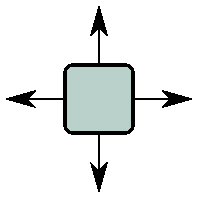
\includegraphics[width=0.2\textwidth]{pics/entite_move}
    \caption{Mouvement autorisé d'une entité}
    \label{move}
\end{figure}

Une entité est soit contrôlée par un joueur ou par l'ordinateur (les humains par exemple).
Chaque entité à un rayon de vision \viewradius{} (commun pour toutes les entités) fixé au début d'une partie.

\begin{figure}[htbp]
    \centering
    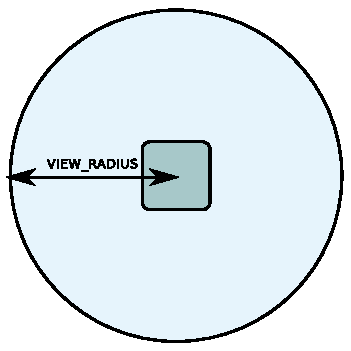
\includegraphics[width=0.4\textwidth]{pics/entite_view}
    \caption{Vision d'une entité}
    \label{view}
\end{figure}

\subsubsection{Les humains} % (fold)
Les humains sont les entités ressources de ce jeu.
Ils sont contrôlés par l'ordinateur et ont un comportement plus ou moins évolué.
Ils n'ont pas de capacité spéciale et tentent d'éviter de se faire contaminer.


% subsubsection Les humains (end)

\subsubsection{Les policiers} % (fold)
Les policiers sont des humains équipés d'une arme à feu.
De ce fait, ils sont capables de tuer les zombies autour d'eux.
Toutefois, leur nombre de balles est limité et ils commencent avec \bulletamount{} balles au début d'une partie.
Une fois que leur stock de balles est épuisé, ils redeviennent de simples humains.

Lorsqu'un zombie est à portée de tir, c'est à dire à une distance inférieure à \shotradius{}, le policier tire automatiquement sur le zombie.
Le tir a une probabilité de chance de réussite de \shotsuccess{}.
Lorsqu'il y a plusieurs zombies à portée, le choix de la cible est aléatoire.

Un policier peut se faire contaminer par un zombie.
Dans ce cas de figure, en plus de la capacité de contaminer des humains, le zombie policier peut tirer sur des zombies adverses.
Comme pour le policier, le tir est automatique et aléatoire si plusieurs zombies sont à portée.

Lorsque le zombie n'a plus de balles, il redevient un zombie comme les autres.


% subsubsection Les policiers (end)

\subsubsection{Les zombies} % (fold)
Les zombies sont les unités que vous controlez.
Elles peuvent\footnote{doivent} contaminer les humains et étendre leur contrôle sur la carte.
Pour cela, chaque zombie dispose d'un compteur de contagions, initialisé à sa création à \contagionamount.
À chaque contagion, ce compteur est décrémenté, ce qui influe sur la prochaine contagion (cf \ref{contagion}).


% subsubsection Les zombies (end)

\subsubsection{Les berzerks} % (fold)
Lorsqu'une contagion ne se passe pas comme désirée (cf \ref{contagion}), l'humain ciblé peut soit mourir, soit devenir un zombie incontrôlable, appelé berzerk.
Un tel zombie est contrôlé par l'ordinateur et ne peut être tué par un policier ou un zombie.
Par contre, il tue zombies et humains autour de lui, lorsqu'il explose, \berzerkdelay{} tours après sa création.
Son explosion tue toutes les entités autour de lui à une distance \berzerkradius{}.

% subsubsection Les berzerks (end)

% subsection Les entités du jeu (end)

\subsection{Les actions du jeu} % (fold)
Une entité (qu'elle soit contrôlée par un joueur ou non) peut se mouvoir dans la carte.
Tous les mouvements ne sont cependant pas possibles. Par exemple, se déplacer vers une case \water.

D'autre part, si deux entités (quelconques) se retrouvent sur la même case à la fin d'un tour, les deux meurent.

% subsection Les actions du jeu (end)

\subsection{Le déroulement d'une partie} % (fold)

Une partie est divisée en plusieurs phases.
Tout d'abord, une phase initiale, où toutes les informations statiques et fixées vous sont fournies.
Ensuite, vient le jeu au tour par tour.

Au début de chaque tour, le joueur a connaissance de :
\begin{itemize}
    \item la position de nouvelles cases de type \water{} découvertes ;
    \item la position des entités, leur type et leur équipe ;
    \item la liste des zombies policiers du joueur qui ont réussi à abattre un autre zombie ;
    \item la liste des zombies du joueur nouvellement créés et quels zombies les ont créés.
\end{itemize}

Le brouillard de guerre s'applique de manière invisible pour le joueur.
On ne lui transmet que les informations qu'il est capable de percevoir.
Une fois qu'un joueur a reçu toutes ces informations, il est capable de décider quelle action fait chacune de ses entités.
Une fois que ce choix est réalisé, on peut exécuter un tour de jeu.


Un tour consiste en la succession d'étapes :

\begin{enumerate}
    \item Déplacer les entités ;
    \item Actions automatiques (tir, explosion berzerk, etc.) ;
    \item Gestion des attaques ;
    \item Gestion des contaminations.
\end{enumerate}

À la fin de chaque tour, on vérifie que les conditions de victoires et de défaites ne sont pas atteintes.
Un joueur est considéré vaincu lorsqu'il n'a plus d'entités sur la carte, que son programme s'est interrompu ou qu'il ne répond plus dans les délais.
Un joueur est considéré vainqueur lorsqu'il est le dernier sur la carte.

Le jeu se termine lorsque un joueur est déclaré vainqueur ou que \turnmax{} tours se sont déroulés (dans ce cas, le score permet de déterminer le vainqueur).

% subsection Le déroulement d'une partie (end)

\subsection{Score d'une partie} % (fold)
Au cours d'une partie, un joueur peut gagner ou perdre des points.
Voici les événements qui influent sur les scores :
\begin{itemize}
    \item Perte d'un zombie = -2 points ;
    \item Humain contaminé = 1 point ;
    \item Zombie tué = 1 point ;
    \item Policier tué = 5 points.
\end{itemize}

% subsection Score d'une partie (end)

\subsection{Contamination d'un humain} % (fold)
\label{contagion}
Lorsqu'un zombie est proche d'un humain (dans un rayon de distance \contagionradius{}), il a des chances de contaminer cet humain.
Dans ce cas de figure, on calcule les probabilités de contamination de la manière suivante :\\
    $$n = \text{compteur de contagions du zombie}$$
    $$P_{contagion} = \frac{n}{\contagionamount}$$

En cas de succès, un nouveau zombie (possiblement policier) est créé et affecté à l'équipe contaminante.
Autrement, l'humain peut soit mourrir soit devenir un berzerk.
La probabilité de créer un berzerk est calculée de la manière suivante :\\
    $$n = \text{compteur de contagions du zombie}$$
    $$P_{berzerk} = \frac{\contagionamount - n}{\contagionamount} * \frac{1}{4}$$

Si plusieurs zombies se situent dans le rayon de contagion d'un humain, on choisit l'équipe la plus représentée puis le zombie ayant un compteur de contagions le plus élevé de cette équipe.
En cas de représentation égale (des équipes) ou de compteurs égaux pour plusieurs zombies, on utilise de l'aléatoire pour choisir l'équipe et/ou le zombie.
Puis les calculs ci-dessus sont réalisés.

Si plusieurs humains se situent autour d'un zombie, l'algorithme ci-dessus est joué pour chacun de ces humains.


% subsection Contamination d'un humain (end)

\subsection{Résolution de combats} % (fold)

Lorsque plusieurs zombies d'équipes différentes sont situés à une distance inférieure ou égale à \attackradius{}, voici comment est déterminé si un zombie est en vie ou non :

\begin{lstlisting}[caption=Résolution de combats, columns=fullflexible]
for every zombie:
        for each enemy in range of zombie:
            if (enemies_in_range(zombie)) >= (enemies_in_range(enemy)) then
                the zombie is marked dead
                /* actual removal is done after all battles are resolved */
                break
    
\end{lstlisting}

% subsection R (end)

\subsection{Distances} % (fold)

Vous avez besoin de manipuler des distances au cours du projet (notamment pour les rayons d'actions).
Dans ce projet, on se basera exclusivement sur la distance euclidienne\footnote{http://en.wikipedia.org/wiki/Euclidean\_distance}.

La distance entre deux points est calculée de la manière suivante :
\begin{center}
    $$ d(p,q) = \sqrt{(p_x - q_x)^2 + (p_y - q_y)^2} $$
    
\end{center}

% subsubsection Distances (end)

\subsection{Disqualification} % (fold)

Un joueur peut être disqualifié pour différentes raisons :
\begin{itemize}
    \item son programme a planté ;
    \item il ne répond plus dans les délais de manière répêtée ;
    \item le programme tente de faire une action jugée illégale.
\end{itemize}

Lorsqu'un joueur est disqualifié, ses entités restent présentes sur la carte mais restent immobiles jusqu'à la fin de la partie (ou leur disparition).

% subsection Disqualification (end)

\subsection{Temps de réponse} % (fold)

À chaque tour, vous avez un temps limite pour choisir les actions de vos entités.
\timinglimit{} désigne cette limite ; elle est fixée au début d'une partie et est valide tout au long d'une partie.

% subsection Temps de réponse (end)

\subsection{Valeurs fixées} % (fold)

Certaines données ont peu de chance de changer entre plusieurs parties.
Elles sont tout de même données en début de parties.
Les voici :

\begin{itemize}
    \item \movelen{} = 1 ;
    \item \viewradius{} = ? ;
    \item \bulletamount{} = 9 ;
    \item \shotradius{} = ? ;
    \item \shotsuccess{} = 50 ;
    \item \contagionamount{} = 9 ;
    \item \contagionradius{} = ? ;
    \item \berzerkdelay{} = 5 ;
    \item \berzerkradius{} = ? ;
    \item \attackradius{} = ? ;
    \item \timinglimit{} = 500ms.
\end{itemize}
% subsection Valeurs fixées (end)


% section Règles (end)

    \lstset{numbers=none}

\section{Spécification du protocole de communication} % (fold)

Cette section décrit la partie technique du projet.
Elle vous permettra de réaliser la partie communication de votre joueur.

Lors d'une partie, plusieurs programmes sont exécutés : le programme des joueurs et un programme (appelé serveur) qui coordonne toutes les actions.
Au début d'une partie, le serveur envoie toutes les informations nécessaires pour le bon déroulement d'une partie (cf \ref{initial}).
Ensuite, à chaque début de tour et pour chaque joueur, le serveur envoie les données courantes et attend en réponse les actions à réaliser (cf \ref{input} et \ref{output}).
Pour finir, une fois qu'une partie se termine pour un joueur (en cas de défaite ou de victoire), le serveur envoie des dernières données au joueur (cf \ref{final}).

\subsection{Serveur de jeu} % (fold)

Le serveur de jeu est un programme qui vous est fourni.
Il permet de lancer des parties, coordonner les joueurs, vérifier les mouvements, vous fournir les données courantes de la partie, etc.
C'est également lui qui gère les entités non jouables (humains, berzerks).
La section \ref{outils} décrit comment utiliser ce serveur de jeu.

La communication avec le serveur de jeu se base sur le protocole TCP\footnote{http://en.wikipedia.org/wiki/Transmission\_Control\_Protocol}.
C'est la forme la plus commune d'échanger des données sur le réseau.
Lorsqu'il s'agit de communiquer en TCP, chaque langage propose son API\footnote{généralement appelé Socket}.
De nombreux exemples peuvent être trouvés sur internet\footnote{par exemple: http://pleac.sourceforge.net}.
Lorsque vous lancez votre programme, vous connaissez l'adresse du serveur et vous êtes donc capable de communiquer avec lui.

\begin{figure}[htbp]
    \centering
    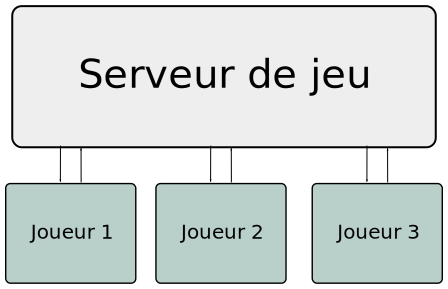
\includegraphics[width=0.5\textwidth]{pics/archi_client_serveur}
    \caption{Architecture Client-Serveur du jeu}
    \label{archi}
\end{figure}

La Figure~\ref{archi} représente le comportement global des programmes lors d'une partie.
Le serveur est le point central et est le seul à avoir la connaissance totale de toutes les données.


% subsection Serveur de jeu (end)

\subsection{Échanges initiaux} % (fold)
\label{initial}
Avant que le jeu ne commence réellement, le serveur et un joueur échangent quelques messages.
Il faut noter que dans tous les échanges suivants, un message commençant par "$<$" sera envoyé du serveur vers le joueur et un message commençant par "$>$" sera envoyé du joueur vers le serveur.
Les mots affichés en bleu sont des mots-clés du protocole.

De plus, les paramètres envoyés en début de partie seront envoyés de la manière suivante: \lstinline!name value!.

\subsubsection{Identification} % (fold)
\label{identification}
Le joueur s'identifie auprès du serveur.

\begin{lstlisting}
>  nick  pseudo
<  nick  pseudo    noPlayer 
\end{lstlisting}

Le pseudo retourné par le serveur n'est pas forcément identique à celui envoyé initialement.
En effet, si deux joueurs donnent le même pseudo, il faut les différencier.
Également, le serveur retourne le numéro d'équipe du joueur.

% subsubsection Identification (end)

\subsubsection{Paramètres de la partie} % (fold)

Les paramètres sont ensuite données de la manière suivante :

\begin{lstlisting}
<  init
<  attack_radius     value
<  berzerk_delay     value
<  berzerk_radius    value
<  bullet_amount     value
<  cols              value
<  contagion_amount  value
<  contagion_radius  value
<  move_len          value
<  nb_team           value
<  rows              value
<  shot_radius       value
<  shot_success      value
<  timing_limit      value
<  turn_max          value
<  view_radius       value
<  end
\end{lstlisting}

Attention, les paramètres ne sont pas forcément donnés dans cet ordre.
De plus, les paramètres peuvent être des flottants ou des entiers.


% subsubsection Paramètres de la partie (end)

% subsection Données initiales et de début de tour (end)

\subsection{Tour par tour : Input} % (fold)
\label{input}

\subsubsection{Données générales} % (fold)
À chaque tour, le serveur actualise les informations du joueur.
Cela commence de la manière suivante :

\begin{lstlisting}
<  turn  turnNo
\end{lstlisting}
\begin{center}
OU
\end{center}
\begin{lstlisting}
<  end
\end{lstlisting}

Dans le deuxième cas, cela annonce que le joueur est vaincu ou bien que la partie est terminée.
Le joueur reçoit alors les données finales (cf \ref{final}).
Si le joueur est toujours en jeu, il reçoit alors les informations courantes de la partie :

\begin{lstlisting}
< players nbPlayersLeft
< scores p1Score ... pnScore
\end{lstlisting}

\subsubsection{Données courantes de la carte} % (fold)

Ensuite, le serveur envoie toutes les données que le joueur peut percevoir.
Ces informations sont formatées de la manière suivante :

\lstset{numbers=left}
\begin{lstlisting}
<  water      row  col
<  entity     row  col     type  team
<  shot       id
<  contagion  id   id_new  row   col   nb_bullets
<  zombie     id   row     col
<  dead       id
\end{lstlisting}
\lstset{numbers=none}


La ligne \lstinline!1! correspond à une case de type \water{} nouvellement découverte à la position \lstinline!(row, col)!.

La ligne \lstinline!2! correspond à la présence d'une entité (d'une autre équipe) à la position \lstinline!(row, col)!.
Cette entité peut être de plusieurs types : \human{}, \cop{}, \zombie{} ou \berzerk{}.
L'entité peut être rattaché à son équipe (par convention, les entités non jouables appartiennent à l'équipe \lstinline!0!).
Un joueur connait son équipe lors de la phase d'identification (cf \ref{identification}).

La ligne \lstinline!3! correspond à une tentative réussie de tir de la part d'un zombie policier \emph{du joueur}.
Le zombie policier est identifié grâce à son \lstinline!id!.

La ligne \lstinline!4! signifie qu'un zombie \emph{du joueur} (identifié par \lstinline!id!) a réussi à contaminer un humain.
Le nouveau zombie (identifié par \lstinline!id_new!) si situe à la position \lstinline!(row, col)!.
Si le nouveau zombie était un humain, \lstinline!nb_bullets! vaudra 0, sinon il vaudra le nombre de balles restantes du policier.

La ligne \lstinline!5! indique que le zombie \emph{du joueur} d'identifiant \lstinline!id! s'est déplacé à la position \lstinline!(row, col)!.
Cette commande est également utilisée lors du premier tour pour placer le ou les zombies initiaux.

La ligne \lstinline!6! désigne un zombie \emph{du joueur} qui est mort au tour précédent.

Lorsque toutes les nouvelles informations sont communiquées au joueur, le serveur notifie le joueur qu'il attend ses instructions :
\begin{lstlisting}
<  end
\end{lstlisting}


% subsubsection Données générales (end)

% subsection Données de chaques tours (end)

\subsection{Tour par tour : Output} % (fold)
\label{output}
Lorsqu'un joueur a reçu toutes les données courantes du tour, il doit prendre des décisions, bouger ou non ses unités.
Pour cela, il peut envoyer au serveur des ordres de mouvement :
\begin{lstlisting}
>  move  id  dir
\end{lstlisting}
Cet ordre consiste de déplacer le zombie \lstinline!id! dans la direction \lstinline!dir!.
La direction peut être égale à \north{}\lstinline!=N!, \east{}\lstinline!=E!, \south{}\lstinline!=S!, \west{}\lstinline!=W!.

Une fois que le joueur a envoyé l'ensemble de ses ordres, il notifie le serveur :
\begin{lstlisting}
>  end
\end{lstlisting}


% subsection Données relatives aux décisions du joueur (end)

\subsection{Données finales} % (fold)
\label{final}

Une fois que le joueur est déclaré vainqueur ou perdant, il reçoit les informations suivantes :

\begin{lstlisting}
<  final   type     turnNo
<  scores  p1Score  ...     pnScore
\end{lstlisting}

Un joueur peut savoir s'il a gagné grâce à \lstinline!type!, qui vaut \lstinline!1! si le joueur est vainqueur, \lstinline!0! sinon.
Pour finir, il peut savoir après combien de tour s'est terminée la partie, grâce à \lstinline!turnNo!.
Les scores finaux sont ensuite transmis au joueur.


% subsection Données finales (end)

% section Spécification (end)

    \section{Outils} % (fold)
\label{outils}

Cette section présentera les outils mis à disposition aux étudiants.
Également, il sera présenté comment utiliser le serveur de jeu en local.

% section Outils (end)

    \section{Recommendations} % (fold)

Afin de vous lancer dans l'implémentation, réfléchissez bien à la conception de votre projet.
Fixez vous des paliers de difficultés progressifs. Ne prenez pas tous les éléments en compte dès le début (policiers, berzerks par exemple).
Vous n'êtes pas non plus obligés de vous servir de toutes les données que l'on vous donne.
Je vous conseille de les prendre en compte au fur et à mesure.

Pour avoir la moyenne (pour la partie code), il vous faudra fournir un programme qui assure une communication correcte avec le serveur et qui adopte une stratégie aléatoire.

% section Conclusion (end)


\end{document}
